\documentclass[%
11pt,%
%oneside,%
twoside,%
%twocolumn,%
titlepage,%
%fleqn,%
%a4page,%
german,%
headsepline%
]{scrartcl}

%\usepackage{fancyhdr}
%\usepackage{scrpage2}
\usepackage{lastpage}
\usepackage{geometry}
\usepackage{graphicx}
\usepackage[utf8]{inputenc}
\usepackage[ngerman]{babel}
\usepackage{lscape}
\usepackage[framemethod=TikZ]{mdframed}
\usepackage[most]{tcolorbox}
\usepackage{mymath}
\usepackage{units}
\usepackage{nicefrac}
\usepackage{pgf,tikz}
\usetikzlibrary{arrows}
\usepackage{colortbl}
\usepackage{hhline}
\usepackage{multirow}
\usepackage[extendedchars]{grffile}
\usepackage{caption}
\usepackage{multicol,calc}
\usepackage{blindtext}
\usepackage{pdfpages}
\usepackage{hyperref}
\usepackage[official]{eurosym}
\usepackage{framed}
\usetikzlibrary{arrows}
\usetikzlibrary{positioning}
\usetikzlibrary{shadows}

%\usepackage{romannum}
\usepackage{longtable}
\usepackage{listings}
\usepackage{wrapfig}

\usepackage{marginnote}
\usepackage[]{qrcode}
\qrset{height=9ex}


% Command, um Tabellen-Spalten anzupassen
\newcommand{\spaltenheight}{\rule{0mm}{3ex}}
\newcommand{\spaltenwidth}{\rule{3cm}{0mm}}
\newcommand{\spaltensep}{\\[1ex]}
%\arrayrulecolor{darkgreen}
\doublerulesepcolor{white}
\definecolor{lightyellow}{rgb}{1,1,0.8}
\definecolor{Gray}{gray}{0.9}


% Pagestyle/Layout
%\geometry{a4paper , tmargin =2.5cm,	bmargin=3cm, lmargin =2.5cm,	rmargin =2.5cm,	headheight=3em, headsep=1em, footskip=1cm}
\setlength{\parindent}{0pt} \setlength{\parskip}{1em}
%für TwoSide
%\lehead{\headmark\pagemark}
%\cehead{}
%\rehead{}
%\lohead{}
%\cohead{}
%\rohead{\headmark}
%für OneSide
%\ihead{}
%\chead{}
%\ohead{}
%\setheadsepline{0.5pt} % Linie zur Begrenzung
%\setfootsepline{0.5pt} % Linie zur Begrenzung
\pagestyle{headings} % gemachte Einstellungen anwenden


\subject{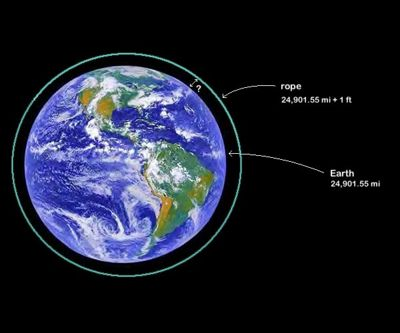
\includegraphics[width=0.618\textwidth]{pictures/rope}}
\title{Lineare Funktionen und Optimierung}
\subtitle{\dots und der Differenzenquotient}
\author{}
\date{}
%\lowertitleback{
%\includegraphics[height=1.1cm]{/Users/jormawassmer/Pictures/logokoeniz.jpg}%
%\copyright Jorma Wassmer
%1. Auflage, Februar 2011
%}


\begin{document}
\maketitle
\tableofcontents
%\thispagestyle{empty}
\cleardoublepage
%\setcounter{page}{1}

\section{Funktionen}
\subsection{Grundlagen}
Aus dem Alltag kennen Sie graphische Darstellungen von Funktionen. Zum Beispiel wird in den Nachrichten der SMI (Swiss Market Index) h\"aufig als Graph illustriert.
\begin{bsp}
\ \\
\begin{center}
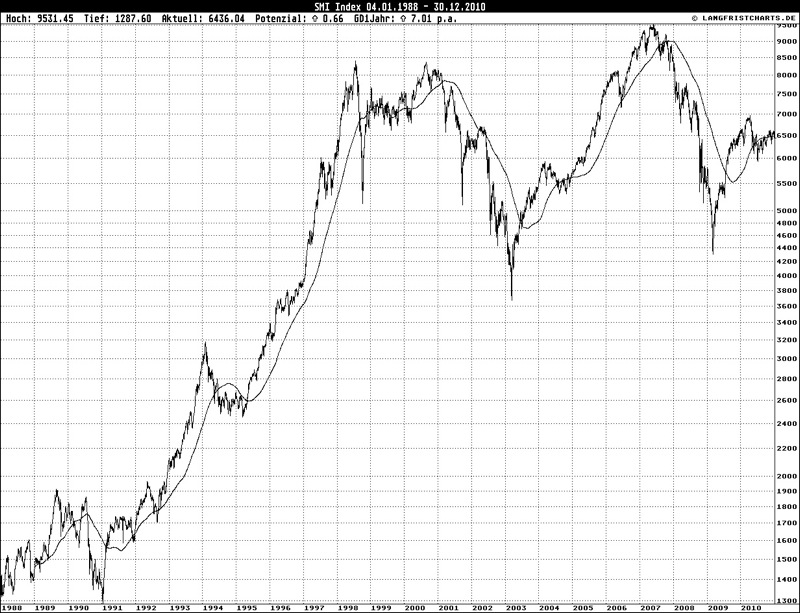
\includegraphics[width=0.7\textwidth]{pictures/smi}
\end{center}
Jedem Datum wird ein bestimmter Index zugeordnet. Den Wert des Index zu einem bestimmten Zeitpunkt kann man auf der vertikalen Achse ablesen.
\end{bsp}
\noindent In der Mathematik versteht man unter einer Funktion folgendes.
\begin{cdef}[Funktion]{}
Eine \emph{Funktion} ist eine Zuordnung, bei der jedem Element $x$ einer Menge $\D{D}$ eindeutig ein Element $y$ einer Menge $\D{W}\subseteq\mathbb{R}$ zugeordnet wird. Man schreibt: $$y=f(x)$$
(sprich:\glqq $y$ gleich $f$ von $x$\grqq)
\end{cdef}
\noindent Anschaulich stellt man eine Funktion mit Mengendiagrammen dar.
\begin{cdef}[Unabhängige Variable, Argument]{}
Die Menge $\D{D}$ nennt man \emph{Definitionsmenge}. Ein Element $x\in\D{D}$ heisst \emph{Argument} von $f$ oder neudeutsch \emph{input}. $x$ wird auch als \emph{unabh\"angige Variable} bezeichnet.
\end{cdef}
\begin{cdef}[Abhängige Variable, Funktionswert]{}
Die Menge $\D{W}$ nennt man \emph{Wertemenge} oder Bild von $f$.  Ein Element $y\in\D{W}$ heisst \emph{Funktionswert} oder neudeutsch \emph{output}. $y$ wird auch h\"aufig als \emph{abh\"angige Variable} bezeichnet.
\end{cdef}
\begin{bsp}
Beim SMI ordnet die Funktion $f$ jedem Monat $x$ genau eine Quote $y$ zu.
\end{bsp}
\begin{bsp}
Das Quadrieren ist eine Funktion. Jeder reellen Zahl $x$ wird ihr Quadrat
$$y=x^2$$
zugeordnet.
\end{bsp}
\subsection{Darstellungen}
Will man beispielsweise als Funktion das Quadrieren von Zahlen darstellen, so kann dies auf verschiedene Arten geschehen. Die gebr\"auchlichsten Darstellungen von Funktionen --- hier am Beispiel des Quadrierens der Werte $-2,-1,0,1,2$ --- sind:
\begin{itemize}
\item Schreibweise konkret mit Funktionswerte:
$f(-2)=4$, $f(-1)=1$, $f(0)=0$, $f(1)=1, f(2)=4$
\item Darstellung als Wertetabelle:
 \begin{center}
  \renewcommand{\arraystretch}{1.2}
  \begin{tabular}{c|rrrrr}
   $x$ & $-2$ &$-1$ & $0$ & $1$ & $2$ \\
   \hline
   $y$ & $4$ & $1$ & $0$ & $1$ & $4$
   \end{tabular}
\end{center}
\item Darstellung als Funktionsgleichung:
$$f(x)=x^2\qq\D{D}=\set{-2,-1,0,1,2}$$
\item graphische Darstellung in einem Koordinatensystem:\\
\begin{figure}[h!]
\begin{center}
\begin{tikzpicture}[line cap=round,line join=round,>=triangle 45,x=0.8cm,y=0.8cm]
\draw[->,color=black] (-4.46,0) -- (5,0);
\foreach \x in {-4,-3,-2,-1,1,2,3,4}
\draw[shift={(\x,0)},color=black] (0pt,2pt) -- (0pt,-2pt) node[below] {\footnotesize $\x$};
\draw[color=black] (4.69,0.06) node [anchor=south west] {$x$};
\draw[->,color=black] (0,-1.5) -- (0,4.49);
\foreach \y in {-1,1,2,3,4}
\draw[shift={(0,\y)},color=black] (2pt,0pt) -- (-2pt,0pt) node[left] {\footnotesize $\y$};
\draw[color=black] (0.07,4.19) node [anchor=west] {$y$};
\draw[color=black] (0pt,-10pt) node[right] {\footnotesize $0$};
\clip(-4.46,-1.5) rectangle (4.92,4.49);
\draw [line width=1.1pt,dotted] (-2,4)-- (0,4);
\draw [line width=1.1pt,dotted] (-2,4)-- (-2,0);
\draw (-3.02,4.7) node[anchor=north west] {$(-2/4)$};
\fill [color=black] (-2,4) circle (1.5pt);
\fill [color=black] (-1,1) circle (1.5pt);
\fill [color=black] (0,0) circle (1.5pt);
\fill [color=black] (1,1) circle (1.5pt);
\fill [color=black] (2,4) circle (1.5pt);
\end{tikzpicture}
\end{center}
\caption{Graphische Darstellung im Koordinatensystem}
\end{figure}
\end{itemize}
\subsection{Graph einer Funktion}
\noindent Wir wollen pr\"azise formulieren, was wir unter dem Graphen einer Funktion verstehen wollen. Zuerst eine Hilfsdefinition
\begin{cdef}[Geordnetes Paar]{}
Ein Paar $\point{x}{y}$ heisst \emph{geordnet}, wenn die Reihenfolge von $x$ und $y$ wesentlich ist.
\end{cdef}
\begin{cdef}[Graph]{}
Sei $f:\D{D}\longrightarrow\D{W}$ eine Funktion. Die Menge aller geordneten Paare
$$G_f=\setm{\point{x}{f(x)}}{x\in\D{D}}$$
heisst \emph{Graph} von $f$.
\end{cdef}
\subsection{Einschr\"ankungen des Definitionsbereichs einer Funktion}
F\"ur manche Beschreibungen von allt\"aglichen Zusammenh\"angen, die als Funktionen beschrieben werden, ist die Anpassung der Definitionsmenge der entsprechenden Funktion sinnvoll. Im Folgenden wird der Einfluss der Definitionsmenge auf die Funktion bzw. ihren Graphen veranschaulicht.
\begin{bsp}
Wir betrachten den Graphen der Funktion
$$f(x)=x^2$$
f\"ur verschiedene Definitionsmengen.\\[2ex]

\begin{center}
\begin{figure}[h!]
\centering
\scalebox{1.5}{
\begin{tikzpicture}[line cap=round,line join=round,>=triangle 45,x=0.7cm,y=0.7cm]
\draw[->,color=black] (-3.28,0) -- (3.22,0);
\foreach \x in {-3,-2,-1,1,2,3}
\draw[shift={(\x,0)},color=black] (0pt,2pt) -- (0pt,-2pt) node[below] {\footnotesize $\x$};
\draw[color=black] (2.99,0.06) node [anchor=south west] { x};
\draw[->,color=black] (0,-0.9) -- (0,6.65);
\foreach \y in {,1,2,3,4,5,6}
\draw[shift={(0,\y)},color=black] (2pt,0pt) -- (-2pt,0pt) node[left] {\footnotesize $\y$};
\draw[color=black] (0.07,6.35) node [anchor=west] { y};
\draw[color=black] (0pt,-10pt) node[right] {\footnotesize $0$};
\clip(-3.28,-0.9) rectangle (3.22,6.65);
\draw[line width=2pt, smooth,samples=100,domain=-3.284975503538376:3.2225095264017423] plot(\x,{(\x)^2});
\end{tikzpicture}
}
\caption{$f:\D{R}\longrightarrow\D{R}$}
\end{figure}
\end{center}
\begin{center}
\begin{figure}[h!]
\centering
\scalebox{1.5}{
\begin{tikzpicture}[line cap=round,line join=round,>=triangle 45,x=0.7cm,y=0.7cm]
\draw[->,color=black] (-3.28,0) -- (3.22,0);
\foreach \x in {-3,-2,-1,1,2,3}
\draw[shift={(\x,0)},color=black] (0pt,2pt) -- (0pt,-2pt) node[below] {\footnotesize $\x$};
\draw[color=black] (2.99,0.06) node [anchor=south west] { x};
\draw[->,color=black] (0,-0.9) -- (0,6.65);
\foreach \y in {,1,2,3,4,5,6}
\draw[shift={(0,\y)},color=black] (2pt,0pt) -- (-2pt,0pt) node[left] {\footnotesize $\y$};
\draw[color=black] (0.07,6.35) node [anchor=west] { y};
\draw[color=black] (0pt,-10pt) node[right] {\footnotesize $0$};
\clip(-3.28,-0.9) rectangle (3.22,6.65);
\fill [color=black] (-1,1) circle (2.0pt);
\fill [color=black] (-2,4) circle (2.0pt);
\fill [color=black] (0,0) circle (2.0pt);
\fill [color=black] (1,1) circle (2.0pt);
\fill [color=black] (2,4) circle (2.0pt);
\end{tikzpicture}
}
\caption{$f:\D{Z}\longrightarrow\D{R}$}
\end{figure}
\end{center}
\begin{center}
\begin{figure}[h!]
\centering
\scalebox{1.5}{
\begin{tikzpicture}[line cap=round,line join=round,>=triangle 45,x=0.7cm,y=0.7cm]
\draw[->,color=black] (-3.28,0) -- (3.22,0);
\foreach \x in {-3,-2,-1,1,2,3}
\draw[shift={(\x,0)},color=black] (0pt,2pt) -- (0pt,-2pt) node[below] {\footnotesize $\x$};
\draw[color=black] (2.99,0.06) node [anchor=south west] { x};
\draw[->,color=black] (0,-0.9) -- (0,6.65);
\foreach \y in {,1,2,3,4,5,6}
\draw[shift={(0,\y)},color=black] (2pt,0pt) -- (-2pt,0pt) node[left] {\footnotesize $\y$};
\draw[color=black] (0.07,6.35) node [anchor=west] { y};
\draw[color=black] (0pt,-10pt) node[right] {\footnotesize $0$};
\clip(-3.28,-0.9) rectangle (3.22,6.65);
\fill [color=black] (1,1) circle (2.0pt);
\fill [color=black] (2,4) circle (2.0pt);
\end{tikzpicture}
}
\caption{$f:\D{N}\longrightarrow\D{R}$}
\end{figure}
\end{center}
\end{bsp}

\begin{ueb}(gerade)
Gegeben sei die Funktion
$$f(x)=-x+2.$$
\begin{enumeratea}
\item Berechne $f(1),f(0)$ und $f(-1)$.
\item Zeichne den Graphen für (i) $f:\mR\rightarrow\mR$ und für (ii) $f:\mN\rightarrow\mR$
\end{enumeratea}
\end{ueb}

\begin{ueb}($x$ hoch 3)
Sei
$$f(x)=x^3.$$
Berechne einige Funktionswerte und skizziere den Graphen.
\end{ueb}

\begin{ueb}(freier Fall)
Gegeben sei die Funktion
$$s(t)=20-5t^2.$$
\begin{enumeratea}
\item Berechne $s(-1),s(0),s(2)$ und $s(2)$
\item Wann gilt $s(t)=0$?
\item Bestimme
\begin{enumeratei}
\item $s(2)-s(1)$
\item $\frac{s(3)-s(1)}{3-1}$
\item $\frac{s(2+h)-s(2)}{h}$
\end{enumeratei}
\item Berechne allgemein für beliebiges $t$ den Quotienten
$$\frac{s(t+h)-s(t)}{h}$$
und überlege dir, welchen Wert dieser Quotient für $h\to0$ annimmt.
\end{enumeratea}
\end{ueb}

\begin{ueb}(exponentiell)
Man weiss von einer Funktion vom Typ
$$N(t)=a\cdot b^t,$$
dass sie die Werte $N(0)=10$ und $N(2)=6.4$ annimmt.
\begin{enumeratea}
\item Bestimme die Parameter $a$ und $b$.
\item Berechne $N(1)$ und $N(-2)$.
\item Skizziere den Graphen.
\item Bestimme
\begin{enumeratei}
\item $\frac{N(2)-N(0)}{2}$
\item $\frac{N(3)-N(1)}{2}$
\item $\frac{N(t+h)-N(t)}{h}$
\end{enumeratei}
\end{enumeratea}
\end{ueb}

\pagebreak

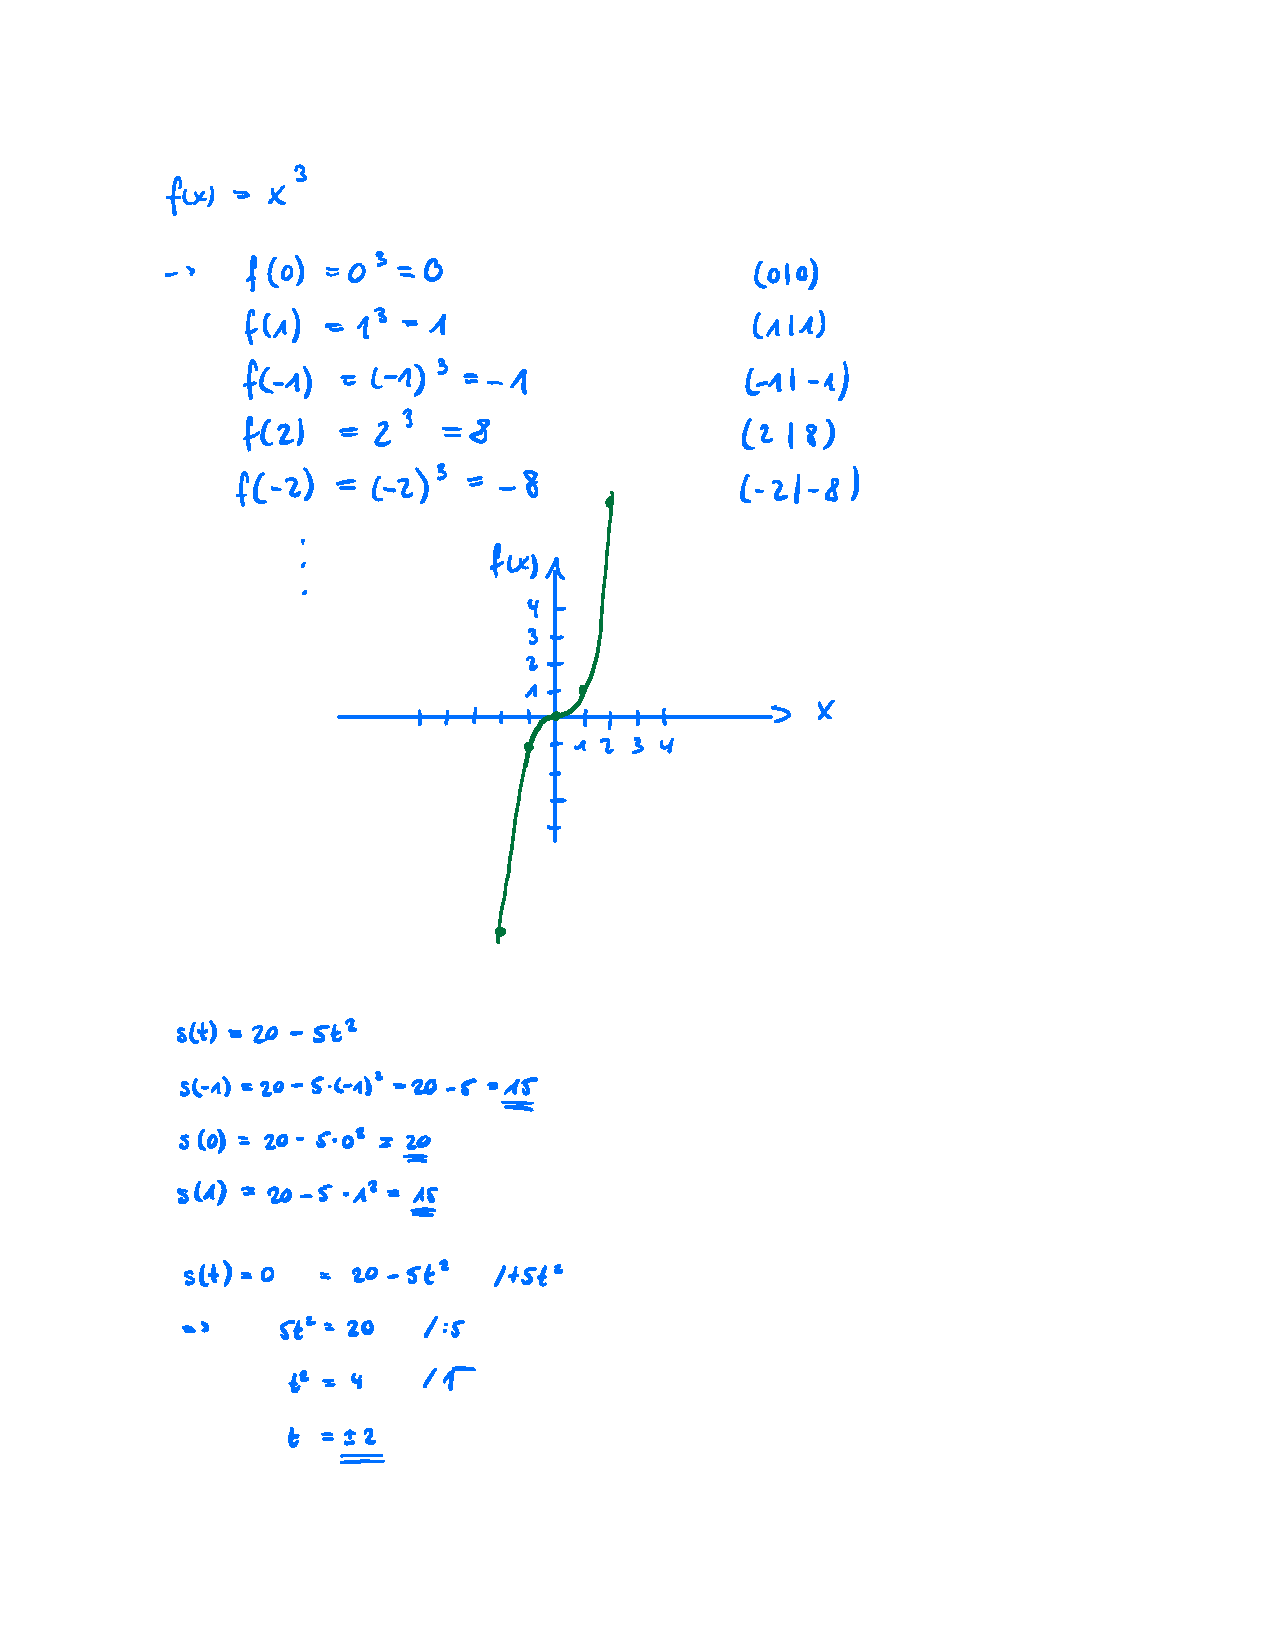
\includepdf[pages={1-3},scale=0.95]{pictures/fktnbasics.pdf}


\pagebreak

\section{Proportionalit\"at}
%\begin{wrapfigure}{r}{0.382\textwidth}
  \begin{center}
    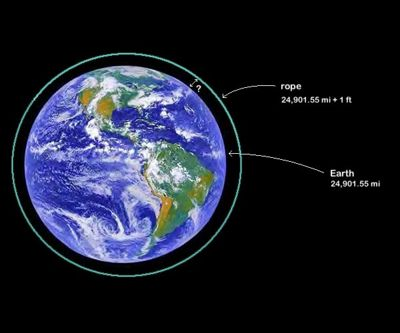
\includegraphics[width=0.618\textwidth]{pictures/rope}
  \end{center}
%\caption{A gull}
%\end{wrapfigure}
Wir betrachten eine spezielle Menge von Funktionen, die Proportionalit\"aten und \glqq umgekehrten\grqq{} Proportionalit\"aten.
\begin{cdef}[Proportionalität]{}
Eine Funktion der Form
$$f(x)=mx\qq m\in\D{R}$$
heisst \emph{Proportionalit\"at}. Der Parameter $m$ heisst \emph{Proportionalit\"atskonstante} oder Proportionalit\"atsfaktor.
\end{cdef}
\begin{bsp}
Die Menge der n\"otigen Zutaten f\"ur ein Rezept in Abh\"angigkeit der Anzahl Essenden ist eine Proportionalit\"at. (Sp\"atzle-Eintopf)
\end{bsp}
\begin{csatz}[Charakteristik Proportionalität]{}
Die zu einer Proportionalit\"at $f$ geh\"orenden Zahlenpaare haben denselben Quo\-tien\-ten.
\end{csatz}
\begin{proof}[Beweis]
Sei $f(x)=mx$ eine Proportionalit\"at. Dann gilt f\"ur beliebige Zahlenpaare
$$\point{x}{y}=\point{x}{mx}$$
und damit f\"ur den Quotienten
$$\frac{y}{x}=\frac{mx}{x}=m$$
\end{proof}
\begin{csatz}[Proportionalität enthält den Ursprung]{}
Der Graph einer Proportionalit\"at ist eine Gerade, die durch den Ursprung verl\"auft; oder eine Teilmenge davon.
\end{csatz}
\begin{proof}[Beweis]
Dass es sich bei Graphen von Proportionalit\"aten um Geraden handelt, werden wir erst in der Tertia beweisen. Dass der Graph durch den Ursprung verl\"auft, sieht man wegen
$$f(0)=m\cdot0=0,$$
d.h. $\point{0}{0}\in G_f$, leicht ein.
\end{proof}
\begin{bsp}
Der Schweredruck $P$ unter Wasser ist proportional zur Tiefe $h$ unter der Wasseroberfl\"ache. Aus der Physik kennt man die Beziehung
$$P(h)=\rho_wgh$$
wobei $\rho_w$ die Dichte von Wasser und $g$ den Ortsfaktor bezeichnet. $P(h)$ ist eine Proportionalit\"at mit Proportionalit\"atskonstante $\rho_wg$.
\end{bsp}
\begin{bem}
Wenn f\"ur die Argumentation bloss wichtig ist, dass es sich um eine Proportionalit\"at handelt und der Wert der Konstanten keine Rolle spielt, schreibt man kurz \glqq$\sim$\grqq. Im obigen Beispiel w\"urde man kurz schreiben
$$P\sim h$$
\end{bem}

\section{Lineare Funktionen}
In diesem Abschnitt werden wir die Menge der Proportionalit\"aten erweitern. Wir erinnern uns daran, dass Proportionalit\"aten die Form $f(x)=mx$ haben und ihre Graphen Geraden --- oder Teilmengen davon --- sind, die durch den Ursprung gehen.
\begin{bsp}
F\"ur ein Handy-Abonnement zahlt man eine Grundgeb\"uhr von $\unit[10]{Franken}$ pro Monat. Jede SMS kostet den Abonnementen $\unit[25]{Rappen}$. Wir stellen die anfallenden Kosten in Abh\"angigkeit der verschickten SMS dar. Dabei gehen wir schrittweise vor und w\"ahlen der Einfachheit halber als Defini\-tions\-menge $\D{D}=\D{R}^+_0$.

\begin{enumeratea}
\item W\"urde man keine Grundgeb\"uhr zahlen, sondern nur die versendeten SMS, dann lautet die Kostenfunktion (Einheiten in Franken)
$$f(x)=0.25x.$$
\begin{center}
\definecolor{cqcqcq}{rgb}{0.75,0.75,0.75}
\scalebox{0.9}{
\begin{tikzpicture}[line cap=round,line join=round,>=triangle 45,x=0.3cm,y=0.3cm]
\draw [color=cqcqcq,dash pattern=on 2pt off 2pt, xstep=0.6cm,ystep=0.6cm] (-1.56,-1.34) grid (18.4,15);
\draw[->,color=black] (-1.56,0) -- (18.4,0);
\foreach \x in {,2,4,6,8,10,12,14,16,18}
\draw[shift={(\x,0)},color=black] (0pt,2pt) -- (0pt,-2pt) node[below] {\footnotesize $\x$};
\draw[color=black] (17.52,0.1) node [anchor=south west] { \# SMS};
\draw[->,color=black] (0,-1.34) -- (0,15);
\foreach \y in {,2,4,6,8,10,12,14}
\draw[shift={(0,\y)},color=black] (2pt,0pt) -- (-2pt,0pt) node[left] {\footnotesize $\y$};
\draw[color=black] (0.1,14.48) node [anchor=west] { Kosten};
\draw[color=black] (0pt,-10pt) node[right] {\footnotesize $0$};
\clip(-1.56,-1.34) rectangle (18.4,15);
\draw[line width=1.5pt, smooth,samples=100,domain=0.0:18.4] plot(\x,{0.25*\x});
\draw[color=black] (4,2) node {$f$};
\end{tikzpicture}
}
\end{center}
\item Mit Grundgeb\"uhr erhalten wir die Kostenfunktion
$$k(x)=0.25x+10$$
\begin{center}
\definecolor{cqcqcq}{rgb}{0.75,0.75,0.75}
\scalebox{0.9}{
\begin{tikzpicture}[line cap=round,line join=round,>=triangle 45,x=0.3cm,y=0.3cm]
\draw [color=cqcqcq,dash pattern=on 2pt off 2pt, xstep=0.6cm,ystep=0.6cm] (-1.56,-1.34) grid (18.4,15);
\draw[->,color=black] (-1.56,0) -- (18.4,0);
\foreach \x in {,2,4,6,8,10,12,14,16,18}
\draw[shift={(\x,0)},color=black] (0pt,2pt) -- (0pt,-2pt) node[below] {\footnotesize $\x$};
\draw[color=black] (17.52,0.1) node [anchor=south west] { \# SMS};
\draw[->,color=black] (0,-1.34) -- (0,15);
\foreach \y in {,2,4,6,8,10,12,14}
\draw[shift={(0,\y)},color=black] (2pt,0pt) -- (-2pt,0pt) node[left] {\footnotesize $\y$};
\draw[color=black] (0.1,14.48) node [anchor=west] { Kosten};
\draw[color=black] (0pt,-10pt) node[right] {\footnotesize $0$};
\clip(-1.56,-1.34) rectangle (18.4,15);
\draw[line width=1.5pt, smooth,samples=100,domain=0.0:18.400000000000002] plot(\x,{0.25*\x+10});
\draw[color=black] (1.6,11.4) node {$k$};
\end{tikzpicture}
}
\end{center}
\end{enumeratea}
\end{bsp}
\noindent Im vorangegangenen Beispiel sieht man, dass die Addition der Grundgeb\"uhr eine Verschiebung des Graphen parallel zur $y$-Achse um $10$ bewirkt:
$$k(x)=0.25x+10=f(x)+10$$
Die Funktion $k$ kann also aus der Proportionalit\"at $f$ durch die Addition einer Konstanten erhalten werden.

\subsection{Mathematische Beschreibung}
\begin{cdef}[Lineare Funktion]{}
Eine Funktion der Form
$$f(x)=mx+b\qq m,b\in\D{R}$$
heisst \emph{lineare Funktion}. Den Parameter $m$ nennt man \emph{Steigung}, den Parameter $b$ Ordinatenabschnitt oder \emph{$y$-Achsenabschnitt}.
\end{cdef}
\begin{bem}
Man erinnere sich an die Definition der Steigung allgemein. Sie ist das Verh\"altnis der H\"ohendifferenz zur Strecke horizontal zwischen zwei Punkten.
\end{bem}
\begin{bem}
Proportionalit\"aten sind spezielle affine Funktionen, n\"amlich affine Funktionen mit $b=0$. In andern Worten: Die Menge der Proportionalit\"aten ist eine Teilmenge der Menge der affinen Funktionen.
\end{bem}
\begin{bem}
Affine Funktionen werden oft f\"alschlicherweise als lineare Funktionen bezeichnet.
\end{bem}
\begin{csatz}[Gerade]{}
Der Graph einer affinen Funktion
$$f(x)=mx+b$$
ist eine Gerade, die die $y$-Achse bei $b$ schneidet.
\end{csatz}
\begin{proof}[Beweis]
Wiederum verschieben wir den Beweis, dass der Graph eine Gerade ist, auf sp\"ater (oder man \"uberlegt sich dies mit einem einfachen \"Ahnlichkeitsargument basierend auf der Definition der Steigung). Der $y$-Achsen-Schnittpunkt liegt wegen
$$f(0)=m\cdot0+b=b$$
im Punkt $\point{0}{b}$.
\end{proof}
\begin{figure}[h!]
\begin{center}
\scalebox{0.8}{
\begin{tikzpicture}[line cap=round,line join=round,>=triangle 45,x=0.6cm,y=0.6cm]
\draw[->,color=black] (-3,0) -- (7.47,0);
\foreach \x in {-2,2,4,6}
\draw[shift={(\x,0)},color=black] (0pt,2pt) -- (0pt,-2pt);
\draw[color=black] (7.21,0.08) node [anchor=south west] { x};
\draw[->,color=black] (0,-1) -- (0,7.83);
\foreach \y in {2,4,6}
\draw[shift={(0,\y)},color=black] (2pt,0pt) -- (-2pt,0pt);
\draw[color=black] (0.08,7.42) node [anchor=west] { y};
\clip(-2.68,-1.3) rectangle (7.47,7.83);
\draw[line width=2pt, smooth,samples=100,domain=-2.6829016613352596:7.470849241564336] plot(\x,{0.5*\x+3});
\draw (0,3)-- (0.36,3);
\draw [line width=1.6pt] (0.21,3)-- (0.21,0);
\draw [line width=1.6pt] (2,4)-- (4,4);
\draw [line width=1.6pt] (4,4)-- (4,5);
\draw (2.95,4) node[anchor=north west] {$1$};
\draw (4.1,4.7) node[anchor=north west] {$m$};
\draw[color=black] (0.5,1.61) node {$b$};
\end{tikzpicture}
}
\end{center}
\caption{Steigung und y-Achsen-Abschnitt}
\end{figure}
\begin{bem}
Weil der Graph einer affinen Funktion eine Gerade ist, reichen zwei Punkte um dessen Funktionsgleichung bestimmen zu k\"onnen bzw. um dessen Graphen skizzieren zu k\"onnen.
\end{bem}
\begin{bem}
Die Information aus letztem Satz ist vor allem hilfreich, um Graphen von affinen Funktionen rasch skizzieren zu k\"onnen. Hat man n\"amlich die Funktionsgleichung
$$f(x)=mx+b$$
gegeben, so kann man den Schnittpunkt des Graphen mit der $y$-Achse direkt ablesen: $\point{0}{b}$. Danach tr\"agt man von dort aus die Steigung ab. Dazu geht man eine Einheit in $x$-Richtung und $m$ Einheiten in $y$-Richtung, was einen zweiten Punkt ergibt. Selbstverst\"andlich kann man auch um mehr als eine Einheit \glqq nach vorne gehen\grqq, wenn die H\"ohe Proportional angepasst wird.
\end{bem}

\subsection{Funktionsgleichung aus zwei gegebenen Punkten bestimmen}
\begin{bsp}
Wir bestimmen die Funktionsgleichung der Geraden, die durch die Punkte $P=\point{-1}{1}$ und $Q=\point{3}{2}$ geht. Weil der Graph eine Gerade ist, muss ihre Funktionsgleichung die Form
$$f(x)=mx+b$$
haben.

Die Differenz der $x$-Werte der beiden Punkte ist $q_x-p_x=3-(-1)=4$ und die der $y$-Werte $q_y-p_y=2-1=1$. Daher ergibt sich f\"ur die Steigung
$$m=\frac{\text{H\"ohendifferenz}}{\text{Strecke horizontal}}=\frac{q_y-p_y}{q_x-p_x}=\frac{1}{4}$$.
\begin{center}
\definecolor{cqcqcq}{rgb}{0.75,0.75,0.75}
\scalebox{1.0}{
\begin{tikzpicture}[line cap=round,line join=round,>=triangle 45,x=1.1cm,y=1.1cm]
\draw [color=cqcqcq,dash pattern=on 3pt off 3pt, xstep=1.1cm,ystep=1.1cm] (-1.5,-1.4) grid (4.6,2.8);
\draw[->,color=black] (-2,0) -- (4.6,0);
\foreach \x in {-2,-1,1,2,3,4}
\draw[shift={(\x,0)},color=black] (0pt,2pt) -- (0pt,-2pt) node[below] {\footnotesize $\x$};
\draw[color=black] (4.5,0.08) node [anchor=south west] { x};
\draw[->,color=black] (0,-1.6) -- (0,3.86);
\foreach \y in {-1,1,2,3}
\draw[shift={(0,\y)},color=black] (2pt,0pt) -- (-2pt,0pt) node[left] {\footnotesize $\y$};
\draw[color=black] (0.1,3.46) node [anchor=west] { y};
\draw[color=black] (0pt,-10pt) node[right] {\footnotesize $0$};
\clip(-2.2,-1.4) rectangle (5.4,4);
\draw [line width=1.2pt,dotted] (-1,1)-- (3,1);
\draw [line width=1.2pt,dotted] (3,1)-- (3,2);
\draw (3.1,1.8) node[anchor=north west] {$q_y-p_y$};
\draw (0.6,1) node[anchor=north west] {$q_x-p_x$};
\fill [color=black] (-1,1) circle (1.5pt);
\draw[color=black] (-1.18,1.4) node {$P$};
\fill [color=black] (3,2) circle (1.5pt);
\draw[color=black] (2.8,2.4) node {$Q$};
\end{tikzpicture}
}
\end{center}
Also m\"ussen wir nur noch den Parameter $b$ bestimmen. Da sowohl $P$ als auch $Q$ Elemente des Graphen sind, erf\"ullen beide die gesuchte Funktionsgleichung. Man nimmt einen der beiden Punkte, z.B. $P$, setzt diesen ein und l\"ost nach $b$ auf:
\begin{align}
f(x)&=\frac{1}{4}x+b\tag{$m=\frac{1}{4}$ einsetzen}\\
1&=\frac{1}{4}\cdot(-1)+b\tag{Punkt $P$ einsetzen}\\
1&=-\frac{1}{4}+b\tag{$+\frac{1}{4}$}\\
\frac{5}{4}&=b\notag
\end{align}
Die Funktionsgleichung der Geraden durch $P$ und $Q$ lautet also:
$$f(x)=\frac{1}{4}x+\frac{5}{4}$$
\end{bsp}

\section{Systeme von linearen Gleichungen}
Wir setzen unser Handy-Abonnement-Beispiel fort.
\begin{bsp}
Wir vergleichen zwei Angebote der Anbieter \glqq Klementine\grqq\ und \glqq SwissPhone\grqq.
\begin{itemize}
\item Klementine bietet ein Abo mit einer Grundgeb\"uhr von $\unit[10]{Franken}$ und jede SMS ˆ $\unit[25]{Rappen}$ an.
\item SwissPhone offeriert eine Grundgeb\"uhr von $\unit[20]{Franken}$ und jede SMS ˆ $\unit[15]{Rappen}$.
\end{itemize}
Frage: Welchen Anbieter w\"ahlen Sie?\\[0ex]

\noindent Wir sch\"atzen Anzahl SMS, die wir pro Monat verschicken, und vergleichen die beiden Anbieter. F\"ur Klementine haben wir die Kostenfunktion
$$k_K(x)=0.25x+10$$
und f\"ur SwissPhone
$$k_S(x)=0.15x+20$$
\vspace*{1ex}
\begin{center}
\definecolor{uququq}{rgb}{0.25,0.25,0.25}
\definecolor{qqqqcc}{rgb}{0,0,0.8}
\definecolor{cczzqq}{rgb}{0.8,0.6,0}
\definecolor{cqcqcq}{rgb}{0.75,0.75,0.75}
\scalebox{1.2}{
\begin{tikzpicture}[line cap=round,line join=round,>=triangle 45,x=0.05cm,y=0.1cm]
\draw [color=cqcqcq,dash pattern=on 1pt off 1pt, xstep=0.5cm,ystep=0.5cm] (-4,-2) grid (125,46);
\draw[->,color=black] (-10,0) -- (128.54,0);
\foreach \x in {20,40,60,80,100,120}
\draw[shift={(\x,0)},color=black] (0pt,2pt) -- (0pt,-2pt) node[below] {\footnotesize $\x$};
\draw[color=black] (119.59,0.41) node [anchor=south west] { \# SMS};
\draw[->,color=black] (0,-4.79) -- (0,50);
\foreach \y in {5,10,15,20,25,30,35,40,45}
\draw[shift={(0,\y)},color=black] (2pt,0pt) -- (-2pt,0pt) node[left] {\footnotesize $\y$};
\draw[color=black] (1.02,47.94) node [anchor=west] { $\nicefrac{Kosten}{Franken}$};
%\draw[color=black] (0pt,-10pt) node[right] {\footnotesize $0$};
\clip(-10,-4.79) rectangle (128.54,50);
\draw[line width=2pt,color=cczzqq, smooth,samples=100,domain=0.0:128.54460093896714] plot(\x,{0.25*\x+10});
\draw[line width=2pt,color=qqqqcc, smooth,samples=100,domain=0.0:128.54460093896714] plot(\x,{0.15*\x+20});
\draw (15.63,30) node[anchor=north west] {$k_S$};
\draw (28.86,17.14) node[anchor=north west] {$k_K$};
\fill [color=uququq] (100,35) circle (1.5pt);
\draw[color=uququq] (99,38) node {$P$};
\end{tikzpicture}
}
\end{center}
Wir sehen, dass ab einer gewissen Anzahl SMS, der urspr\"unglich teurere Anbieter SwissPhone billiger ist als Klementine. Deshalb wollen wir die Anzahl SMS bestimmen, f\"ur den die Kosten bei beiden Anbietern gleich ausfallen. In andern Worten: Wir bestimmen denjenigen $x$-Wert, f\"ur den
$$k_K(x)=k_S(x)$$
gilt. Dies ist gerade der Schnittpunkt $P$ der Graphen der beiden Funktionen.
Wir erhalten
\begin{align}
k_K(x)&=k_S(x)\tag{Bedingung Schnittpunkt}\\
0.25x+10&=0.15x+20\tag{$-0.15x-10$}\\
0.1x&=10\tag{$\cdot10$}\\
x&=100\notag
\end{align}
F\"ur $100$ verschickte SMS pro Monat sind beide Anbieter gleich teuer; die Kosten betragen dann
$$k_K(100)=0.25\cdot100+10=\unit[35]{Franken}$$
Das heisst, ab $101$ verschickten SMS pro Monat ist SwissPhone billiger.
\end{bsp}
In der vorangegangenen Aufgabe lag das Kernproblem darin, f\"ur beide Funktionen ein Paar $\point{x}{y}$ zu bestimmen, dass beide Funktionsgleichungen gleichzeitig erf\"ullt. Weiter erkannten wir, dass diese L\"osung der Schnittpunkt der Graphen der beiden Funktionen ist. Im Folgenden werden Methoden vorgestellt, wie man solche L\"osungen berechnen kann.

\subsection{Systeme mit 2 linearen Gleichungen und 2 Unbekannten}
Wir stellen uns bildlich die wichtigsten Begriffe bereit, ohne daf\"ur die mathematisch korrekten Definitionen zu verwenden.

Gleichungen, die zusammen betrachtet werden sollen, nennt man ein System von Gleichungen. Grunds\"atzlich gilt, dass man so viele Gleichungen braucht, wie maximal Variablen auftauchen, um ein System von Gleichungen numerisch l\"osen zu k\"onnen. Eine Gleichung heisst linear, wenn jede Variable separat mit dem Exponenten $1$ vorkommt.
\begin{bsp}
Eine lineare Gleichung ist zum Beispiel
$$x+2y+\sqrt{3}z=5^3$$
Hingegen sind
$$x+y^2+\sqrt{z}=5^3$$
und
$$x+yz=5^3$$
keine linearen Gleichungen.
\end{bsp}

Zuerst betrachten wir den einfachsten Fall, n\"amlich ein System von zwei Gleichungen mit zwei Unbekannten.
\begin{bsp}
Gegeben seien die beiden Gleichungen
\begin{align}
y+2x&=1\\
y-x&=-5
\end{align}
Dies ist ein System von zwei linearen Gleichungen mit zwei Unbekannten.
\end{bsp}
Es gibt nun verschiedene Methoden, die L\"osung $\point{x}{y}$ dieses Systems zu berechnen. Bevor wir aber die L\"osung bestimmen, \"uberlegen wir uns, wie viele L\"osungen f\"ur ein beliebiges System von zwei linearen Gleichungen mit zwei Unbekannten existieren k\"onnen:
\begin{quote}
Wir k\"onnen annehmen, dass in beiden Gleichungen beide Variablen $x$ und $y$ auftauchen. (Ansonsten w\"urden wir einfach diejenige mit nur einer Unbekannten nehmen, nach dieser  aufl\"osen, in die andere einsetzen und h\"atten nun bloss noch eine Gleichung mit einer Unbekannten.) Wenn beide Variablen vorkommen, l\"ost man beide Gleichungen nach $y$ auf und kann sie als affine Funktionen interpretieren:
\begin{align}
y&=-2x+1\tag{$1'$}\\
y&=x-5\tag{$2'$}
\end{align}
Da die L\"osungen den Schnittpunkten der beiden zugeh\"origen Geraden entsprechen k\"onnen drei F\"alle eintreten:
\begin{itemize}
\item Die Geraden schneiden sich in einem Punkt.
\item Die Geraden sind Parallel und verschieden.
\item Die Geraden fallen zusammen.
\end{itemize}
\noindent Daher kann es eine, keine bzw. unendlich viele L\"osungen geben.
\end{quote}

\subsection{L\"osungsmethoden}
\subsubsection{Gleichsetzungsmethode}
Um unser Gleichungssystem
\begin{align}
y+2x&=1\tag{1}\\
y-x&=-5\tag{2}
\end{align}
zu l\"osen, k\"onnen wir beide Gleichungen separat nach einer der beiden Variablen aufl\"osen, zum Beispiel nach $y$:
\begin{align}
y&=-2x+1\tag{$1'$}\\
y&=x-5\tag{$2'$}
\end{align}
Anschliessend setzt man die beiden gleich und l\"ost auf:
\begin{align}
-2x+1&=x-5\tag{$+2x+5$}\\
6&=3x\tag{$\div3$}\\
2&=x\notag
\end{align}
Die L\"osung $x=2$ setzt man nun in einer der beiden Gleichungen ein, um $y$ zu bestimmen:
$$y=2-5=-3$$
Das heisst, das Zahlenpaar $\point{2}{-3}$ ist L\"osung des Gleichungssystems $(1), (2)$.

\subsubsection{Substitutionsmethode}
Man w\"ahlt eine der beiden Gleichungen
\begin{align}
y+2x&=1\tag{1}\\
y-x&=-5\tag{2}
\end{align}
aus und l\"ost diese, zum Beispiel (1), nach einer Variablen auf, hier nach $y$:
\begin{equation}
y=-2x+1\tag{1'}
\end{equation}
Danach ersetzt man in der andern Gleichung die Variable durch den gewonnenen Term und l\"ost auf:
\begin{align}
y-x&=-5\tag{1') in (2}\\
-2x+1-x&=-5\tag{$-1$}\\
-3x&=-6\tag{$\div(-3)$}\\
x&=2\notag
\end{align}
Schliesslich setzt man die L\"osung $x=2$ in eine der Gleichungen ein und erh\"alt
$$y=-2\cdot 2+1=-3$$
also $\point{2}{-3}$ als L\"osung.

\subsubsection{Additionsmethode}
Bei dieser Methode addiert man beide Gleichungen miteinander oder subtrahiert eine Gleichung von der andern. Dabei pr\"apariert man die Gleichungen vorher so, dass mindestens eine Variable in beiden Gleichungen bis auf Vorzeichen denselben Koeffizienten hat.

Ich demonstriere die Methode auf zwei Arten. Beim Gleichungssystem
\begin{align}
y+2x&=1\tag{1}\\
y-x&=-5\tag{2}
\end{align}
kann ich direkt $(2)$ von $(1)$ subtrahieren.
\begin{equation}
3x=6\tag{$2)-(1$}
\end{equation}
und erhalte $x=2$ und daraus $y=-3$.

Will ich aber gleiche Koeffizienten vor dem $x$, dann multipliziere ich die Gleichung $(2)$ mit $2$.
\begin{align}
y+2x&=1\tag{1}\\
2y-2x&=-10\tag*{$2\cdot(2)$}
\end{align}
und addiere die beiden Gleichungen.
\begin{equation}
3y=-9\tag{$1)+(2$}
\end{equation}
Das heisst $y=-3$ und erh\"alt unmittelbar $x=2$.
\begin{bem}
Alle Methoden f\"uhren nat\"urlich bei gegebenem Gleichungssystem auf die selbe L\"osung.
\end{bem}
\begin{bem}
Die oben aufgef\"uhrten Methoden sind auch auf Systeme von $n$ linearen Gleichungen mit $n$ L\"osungsvariablen anwendbar. Dabei wird jeweils pro eine Ausf\"uhrung eine Variable eliminiert. So kann man sukzessive die Anzahl Variablen und Gleichungen reduzieren, bis schliesslich eine Gleichung mit einer Unbekannten \"ubrig bleibt, die man l\"ost. Danach k\"onnen r\"uckw\"arts schrittweise alle vorhandenen Variablen berechnet werden. Dieses Vorgehen wird im n\"achsten Abschnitt f\"ur drei Gleichungen mit drei Unbekannten demonstriert.
\end{bem}

\subsection{Systeme von 3 linearen Gleichungen mit 3 Unbekannten}
Ich demonstriere das Vorgehen zum L\"osen an folgendem Gleichungssystem. Ziel ist es, bei jeder Kombination von Gleichungen aus dem System eine Variable zu eliminieren.
\begin{bsp}
Gegeben sei das Gleichungssystem
\begin{align}
2x+3y-4z&=-5\tag{1}\\
3x-5y+2z&=4\tag{2}\\
4x+\phantom{1}y-2z&=5\tag{3}
\end{align}
Ich w\"ahle die Additionsmethode, weil die Koeffizienten der Variable $z$ danach schreien. Die Additionen $(2)+(3)$ und $(1)+2\cdot(2)$ vereinfachen das System auf $2$ Gleichungen mit $2$ Unbekannten.
\begin{align}
7x-4y&=9\tag{4}\\
8x-7y&=3\tag{5}
\end{align}
und $z$ ist eliminiert. F\"ur das weitere Vorgehen w\"ahle ich erneut die Additionsmethode und pr\"apariere die Gleichungen so, dass $y$ eliminiert werden kann. $7\cdot(4)$ und $4\cdot(5)$ liefert
\begin{align}
49x-28y&=63\tag{4'}\\
32x-28y&=12\tag{5'}
\end{align}
und $(4')-(5')$ liefert noch eine Gleichung mit einer Unbekannten.
\begin{align}
17x&=51\tag*{$\div17$}\\
x&=3\tag{6}
\end{align}
Nun setzt man $x=3$ ein um die Werte f\"ur $y$ und $z$ zu erhalten.
\begin{align}
21-4y&=9\tag{6) in (4}\\
12&=4y\tag*{$\div4$}\\
3&=y\tag{7}
\end{align}
Wir kennen $x=3$ und $y=3$ und berechnen $z$ mit Gleichung $(1)$.
\begin{align}
6+9-4z&=-5\tag{6) und (7) in (1}\\
20&=4z\tag*{$\div4$}\\
5&=z\tag{8}
\end{align}
Damit erhalten wir die L\"osung $\pointd{3}{3}{5}$.
\end{bsp}
\begin{bem}
Die Form der obigen L\"osung, $\pointd{x}{y}{z}$, heisst Zahlentripel.
\end{bem}

\begin{ueb}(GlSys 3)
  Wir l\"osen das Gleichungssystem
  \begin{align}
    2x+3y+4z&=1.4\qquad(1)\notag\\
    3x-2y-z&=1.2\qquad(2)\notag\\
    5x+4y+3z&=1.4\qquad(3)\notag
  \end{align}
\end{ueb}

\subsection{Regeln zum L\"osen von Gleichungssystemen}
Beim L\"osen von $n$ Gleichungen mit $n$ Unbekannten geht man wie
folgt vor:

\begin{enumerate}
  \item Reduktion
  \begin{enumerate}
    \item[1.] Aus dem Ausgangssystem stellt man mittels Koeffizienten-
    oder Substitutionsmethode ein Gleichungssystem von $n-1$
    Gleichungen mit $n-1$ Unbekannten her.
    \item[2.] Auf analoge Weise bestimmt man daraus ein Gleichungssystem
    von $n-2$ Gleichungen mit $n-2$ Unbekannten und f\"ahrt so fort,
    bis man
    \item[n.] eine Gleichung mit einer Unbekannten hat.
  \end{enumerate}
  \item L\"osungen
  \begin{enumerate}
    \item[1.] Man l\"ost die erhaltene Gleichung mit einer Unbekannten.
    \item[2.] Man setzt die im 1. Schritt erhaltene L\"osung in eine
    Gleichung mit $2$ Unbekannten ein und f\"ahrt so fort, bis man
    \item[n.] die $n$. Unbekannte bestimmt hat.
  \end{enumerate}
  \item Kontrolle
\end{enumerate}

\noindent Stichwort $\rightarrow$ ReL\"oKo

\begin{ueb}(GlSys 4)
  L\"osen Sie das Gleichungssystem
  \begin{align}
    x+4y-z&=6\phantom{1}\qquad(1)\notag\\
    y+4z-u&=10\qquad(2)\notag\\
    -x+z+4u&=18\qquad(3)\notag\\
    4x-y+u&=6\phantom{1}\qquad(4)\notag
  \end{align}
\end{ueb}

\clearpage

\appendix

\section{Weitere Kommentare und Übungen zu linearen Funktionen und Gleichungen}

\subsection{Begriffe und Beispiele}

Eine \textbf{lineare Gleichung} ist eine Gleichung, in der die gesuchte Zahl $x$ nur mit einer anderen Zahl, festen multipliziert wird, und eine weitere Zahl addiert wird, etwa $$3x-12=0$$ Die Gleichung $$x^2+x-1=0$$ hingegen ist \emph{keine} linear Gleichung, da das $x$ in der Potenz $2$ vorkommt. Die Gleichungen $$\frac{2}{x}-1=0$$ und $$3\sqrt{x}-4=2$$ sind ebenfalls keine lineare Gleichungen.

Im allgemein wir jede Gleichung linear genannt, welche auf die Form $$\boxed{a\cdot x + b = 0}$$ gebracht werden kann, wobei $a$ und $b$ fest Werte sind. Im Prinzip können Terme $x^2$, $\frac{1}{x}$, $\sqrt{x}$, und weitere kompliziertere Terme schon vorkommen, müssen aber durch geschicktes Umformen eliminiert werden können. Zum Beispiel, die Gleichung $$x^2+3x-1=x^2$$ kann durch subtrahieren von $x^2$ auf beiden Seiten des Gleichheitszeichen auf die lineare Gleichung $$3x-1=0$$ zurückgeführt werden.

Wie lassen sich lineare Gleichungen lösen? Immer nach dem selben Prinzip: \emph{"Bringe $x$ auf die eine Seite, und die Zahlen auf die andere Seite des Gleichheitszeichen."} 

\begin{bsp}
Die Gleichung $$3x-4 = 0$$ kann wie folgt gelöst werden:
\begin{align*}
3x -4 & = 0 \quad| \, +4\\
3x & = 4 \quad| \, :3\\
x & ={\frac{4}{3}}\\ 
\end{align*}
\end{bsp}

Manchmal ist, wie oben schon erwähnt, die Linearität der Gleichung versteckt, und es muss durch Umformen zuerst in die richtige Form gebracht werden. Wir geben vier typische Beispiele:

\begin{bsp} Die Variabel $x$ ist auf beiden Seiten des Gleichheitszeichen: $$0.5 x-3 = 2 x+1$$ Wiederum, bringe alle $x$ auf die eine Seite, und alle Zahlen auf die andere Seite des Gleichheitszeichen:
                \begin{align*}
                0.5 x-3 & = 2 x+1 \quad| \, -2x\\
                -1.5 x -3 & = 1 \quad| \, +3\\
                -1.5 x & =4 \quad| \, : -1.5\\
                x & = \frac{4}{-1.5}={-2.\overline{6}}
                \end{align*}
\end{bsp}

\begin{bsp}
                Manchmal sind mehrere $x$ auf beiden Seiten, und mehr als eine Zahl $$0.5 x-3 +4x +5 = 2.4 x+1 -3x+2-6x$$ Dann gilt es, die beiden Seiten zuerst zu vereinfachen, daher die $x$-en und Zahlen zusammenzufassen. Erinnere dich daran, wie die $x$-e zusammengefasst werden. Zum Beispiel, betrachte den algebraischen Ausdruck $3x+0.5x$. Wir können die Zusammenfassen zu $3x+0.5x=3.5x$. Warum? Denke an Äpfel: $3$ Äpfel und $0.5$ Äpfel sind $3.5$ Äpfel. Der formale Weg geht wie folgt: $$3x+0.5x=x(3+0.5)=x\cdot 3.5=3.5x$$ Wir lösen nun die Gleichung:
                \begin{align*}
                0.5 x-3 +4x +5& = 2.4 x+1 -3x+2-6x\quad| \, simplify\\
                4.5 x +2 & = -6.6x +3 \quad| \, +6.6x\\
                11.1 x +2 & = 3 \quad| \, -2\\
                11.1 x & =1 \quad| \, :11.1\\
                x & = \frac{1}{11.1}={0.09009...}
                \end{align*}
\end{bsp}           

\begin{bsp} Die rechte und/oder linke Seite enthält $x^2$ oder andere Potenzen $$2x^2+4x-3 =  2-x+2x^2$$ Im Moment ist die einzigen Hoffnung, dass sich diese Terme wegkürzen. Hier ist eine Beispiel:
                \begin{align*}
                2x^2+4x-3 &=  2-x+2x^2 \quad| \, -2x^2\\
                4x -3 & = 2-x \quad| \, +x\\
                5x -3 & = 2 \quad| \, +3\\
                5x & = 5 \quad| \, :5\\
                x & ={1}\\
                \end{align*}
\end{bsp}           

\begin{bsp} Das $x$ erscheint im Nenner eines Bruchs $$\frac{4}{x}-3 = 2$$ Die idee hier ist, beide Seiten mit $x$ zu multiplizieren, damit wir das $x$ im dem Nenner wegbringen: 
                \begin{align*}
                \frac{4}{x}-3 &= 2  \quad| \, +3\\
                \frac{4}{x} & = 5 \quad| \, \cdot x\\
                4 & =  5x\quad| \, :5\\
                {\frac{4}{5}}& = x  
                \end{align*}
                Beachte, dass wir schon im ersten Schritt beide Seiten mit $x$ multiplizieren könnten:
                \begin{align*}
                \frac{4}{x}-3 &= 2  \quad| \, \cdot x\\
                x\cdot (\frac{4}{x}-3) & = 2x \\
                4-3x & = 2x \quad| \, +3x\\
                4 & =  5x\quad| \, :5\\
                {\frac{4}{5}}& = x  
                \end{align*}
\end{bsp}

\subsection{Übungen}

\begin{ueb} Falls linear, löse die Gleichung nach $x$ auf.
                \begin{enumerate}[a)]
                                \item $6x-10=x-5$
                                \item $-x-2=x+3$
                                \item $3-4x=5-2x-16$
                                \item $15x-73-24x=59-16+20x$
                                \item $56x-43-52-19x=7-72x-56x+165x-112$
                                \item $92-13x-x^2=52-3x-x^2$
                                \item $14-(10-x)=0$
                                \item $14-(x-15)=2-(6x+13)$
                                \item $5(4x+9)-6(2x-5)=75$
                                \item $10-6(x-14)=20-3(2x-25)$
                                \item $(15x-3)^2=x(225x-15)$
                                \item $(x-5)(x-2)=(x-4)(x-3)$
                                \item $(x+3)(x-5)=(x-3)^2$
                                \item $x^2-3x+14=x(x+7)$
                                \item $(2x-3)^2=(2x+3)^2+12$
                                \item $\frac{x}{4}+\frac{1}{5}=\frac{x}{2}+\frac{x}{6}$
                                \item $\frac{x+3}{5}=\frac{2x-8}{3}$
                                \item $\frac{3}{x}+1 = 2$
                                \item $\frac{7}{x}-4 = \frac{2}{x}+2$
                                \item $\frac{2}{x}+x = x+7$  
                \end{enumerate}
\end{ueb}

\begin{ueb} Finde die Gleichung, und löse sie.
                \begin{enumerate}[a)]
                                \item Die Summe fünf aufeinander folgenden natürlichen Zahlen ist $960$. Finde diese Zahlen.
                                \item Die Differenz zweier natürlichen Zahlen ist $3$, die Differenz der Quadrate $381$. Finde diese Zahlen.
                                \item Eine Treppe in den ersten Stock hat $22$ Stufen. Würde jede Stufenhöhe um $1.6 cm$ erhöht, bräuchte es nur $20$ Stufen. Wie hoch sind die Treppenstufen?
                                \item Ein Baum hat die Höhe $2.5 m$ ist irgendwo in der Mitte gebrochen, und zwar so, dass der obere Teil nun den Boden $50 cm$ entfernt vom Stamm berührt. Auf welche Höhe ist die Bruchstelle des Baums?
                                \item Ein Zug mit Geschwindigkeit $72 km/h$ verlässt den Bahnhof $A$ um $15:00$ und fährt Richtung Bahnhof $B$. Um $15:15$ fährt ein andere Zug mit Geschwindigkeit $88km/h$ vom Bahnhof $B$ in Richtung $A$. Die Distanz zwischen $A$ und $B$ betrage $120 km$. Wann kreuzen sich die Züge?
                                \item Hahnen 1 füllt den Pool in 1 Stunde, Hahnen 2 in 2 Stunden, Hahnen 3 in 3 Stunden, und Hahnen 4 in 4 Stunden. Wie lange dauert es den Pool zu füllen, wenn alle Hahnen gleichzeitig aufgedreht werden?
                \end{enumerate}
\end{ueb}

{
\subsection{Lösungsskizzen}
                Aufgabe 1: Nicht alle Schritte sind aufgeschrieben ... 
                \begin{enumerate}[a)]
                                \item $6x-10=x-5 \rightarrow 5x=5 \rightarrow x={1}$
                                \item $-x-2=x+3 \rightarrow 2x=-5 \rightarrow x={-2.5}$
                                \item $3-4x=5-2x-16 \rightarrow 2x=14 \rightarrow x={7}$
                                \item $15x-73-24x=59-16+20x  \rightarrow -29x=116  \rightarrow x={-4}$
                                \item $56x-43-52-19x=7-72x-56x+165x-112  \rightarrow 0 = 10 (?)\rightarrow {no\, solution}$
                                \item $92-13x-4x^2=52-3x-4x^2 \rightarrow 10x=40\rightarrow x={4}$
                                \item $14-(10-x)=0 \rightarrow 4+x=0 \rightarrow x={-4} $
                                \item $14-(x-15)=2-(6x+13) \rightarrow -x+29= -6x-11 \rightarrow 5x = -40 \rightarrow x={-8}$
                                \item $5(4x+9)-6(2x-5)=75 \rightarrow 20x+45 -12x+30 = 75 \rightarrow \rightarrow 8x=0 \rightarrow x={0}$
                                \item $10-6(x-14)=20-3(2x-25) \rightarrow 10-6x+84 = 20-6x+75 \rightarrow 94=95(?) \rightarrow {no \, solution}$
                                \item $(15x-3)^2=x(225x-15) \rightarrow 225x^2-90x+9 = 225x^2-15x \rightarrow 75x = 9 \rightarrow x={0.12}$
                                \item $(x-5)(x-2)=(x-4)(x-3)\rightarrow x^2-7x+10 = x^2-7x+12 \rightarrow 10=12(?) \rightarrow {no \, solution}$
                                \item $(x+3)(x-5)=(x-3)^2\rightarrow x^2-2x-15 = x^2-6x+9 \rightarrow 4x=24  x={6}$
                                \item $x^2-3x+14=x(x+7)\rightarrow x^2-3x+14=x^2+7x \rightarrow 10x=14 \rightarrow x={1.4}$
                                \item $(2x-3)^2=(2x+3)^2+12\rightarrow 4x^2 -12x+9 = 4x^2+12x+9+12\rightarrow -24x=12 \rightarrow x={-0.5}$
                                \item $\frac{x}{4}+\frac{1}{5}=\frac{x}{2}+\frac{x}{6}\rightarrow \frac{x}{4}-\frac{x}{2}-\frac{x}{6} = -\frac{1}{5} \rightarrow  \frac{3x-6x-2x}{12}=-\frac{1}{5} \rightarrow \frac{-5x}{12}=-\frac{1}{5}\rightarrow x=\frac{12}{25}={0.48}$
                                \item $\frac{x+3}{5}=\frac{2x-8}{3}\rightarrow x+3 = \frac{5(2x-8)}{3}\rightarrow 3(x+3)=5(2x-8) \rightarrow 3x+9=10x-40 \rightarrow 7x=49 \rightarrow x={7}$
                                \item $\frac{3}{x}+1 = 2\rightarrow \frac{3}{x}=1\rightarrow x={3}$
                                \item $\frac{7}{x}-4 = \frac{2}{x}+2\rightarrow \frac{5}{x}=6 \rightarrow 6x=5 \rightarrow x={0.8\overline{3}}$
                                \item $\frac{2}{x}+x = x+7\rightarrow 2+x^2 = x^2+7x \rightarrow 7x=2 \rightarrow x={\frac{2}{7}}$  
                \end{enumerate}
                Aufgabe 2:
                \begin{enumerate}[a)]
                                \item Es sei $x$ die kleinste dieser Zahlen. Die fünf Zahlen sind also $x$, $x+1$, $x+2$, $x+3$, $x+4$. Die Summe ist $960$, also $$x+(x+1)+(x+2)+(x+3)+(x+4)=960$$ whas wir vereinfachen zu $${5x+10=960}$$ Die Lösung ist $$x=\frac{950}{5}={190}$$ Kontrolle: $190+191+192+193+194=960$
                                \item Es sei $x$ die kleinere der zwei Zahlen. Die grössere Zahl ist also $x+3$, da die Differenz $3$ sein muss. Wir erhalten die Gleichung $${(x+3)^2-x^2=381}$$ Um sie zu lösen, zuerst ausmultiplizieren
                                \begin{align*}
                                (x+3)^2-x^2 & =381 \\
                                {x^2}+6x+9 -{x^2} & = 381 \quad | \, -9\\
                                6x & = 372 \quad | \, :6\\
                                x & =\frac{372}{6}={62}\\ 
                                \end{align*}
                                Kontrolle: $65^2-62^2=381$.
                                \item Zeichne die Situation! 
                                %\begin{center}\includegraphics[scale=0.20]{steps_sol}\end{center}
                                Die Gleichung ist wie folgt, wobei $x$ die original Stufenhöhe ist: $${20  (x+1.6) = 22x}$$ Auflösen nach $x$:
                                \begin{align*}
                                20  (x+1.6) & = 22x \\
                                20x+32 & = 22x \quad | \, -20x\\
                                32 & = 2x \quad | \, :2\\
                                {16} & =x 
                                \end{align*}
                                Die originale Stufenhöhe ist also $16 cm$.
                                \item Zeichen die Situation!
                                %\begin{center}\includegraphics[scale=0.20]{tree_sol}\end{center}
                                Es wird die folgenden Gleichung erhalten, wobei $x$ die Höhe der Bruchstelle ist (in $cm$): $${x^2+50^2 = (250-x)^2}$$ Die Lösung ist
                                \begin{align*}
                                x^2+50^2 & = (250-x)^2 \\
                                x^2+2500 & = 250^2-500x+x^2 \quad | \, -x^2\\
                                2500 & = 62\,500-500x \quad | \, -62\,500\\
                                -60\,000 & = -500x \quad | \, : (-500)\\
                                {120} & =x 
                                \end{align*}
                                Die Höhe der Bruchstelle ist $120 cm=1.2 m$.
                                \item Zeichne die Situation, wobei $t$ die Zeit in Stunden ist, die die vergangene Zeit seit $15:15$ misst.  %\begin{center}\includegraphics[scale=0.20]{train_sol}\end{center} 
                                Die Gleichung ist ${102-160 t = 0}$, und somit $t=\frac{102}{160}=0.6375 h = 38.25 min$. Die Züge kreuzen sich also um ${15:53 \mbox{ and } 15 \mbox{ seconds}}$.
                                \item Das Volumen des Pools sein $V$. Wir haben dann\\
                                \begin{tabular}{lllllll}
                                                Hahnen 1 & $\rightarrow$ &  $1\,h \mbox{ füllt } V$ & $\rightarrow$ & & $\rightarrow$ & $x\, h \mbox{ füllt } x\cdot V$\\
                                                Hahnen 2 & $\rightarrow$ &  $2\,h \mbox{ füllt } V$ &$\rightarrow$ &$1\,h \mbox{ füllt } \frac{1}{2} V$ & $\rightarrow$ & $x\, h \mbox{ füllt } \frac{x}{2}\cdot V$\\
                                                Hahnen 3 & $\rightarrow$ &  $3\,h \mbox{ füllt } V$ &$\rightarrow$ &$1\,h \mbox{ füllt } \frac{1}{3} V$ & $\rightarrow$ & $x\, h \mbox{ füllt } \frac{x}{3}\cdot V$\\
                                                Hahnen 4 & $\rightarrow$ &  $4\,h \mbox{ füllt } V$ &$\rightarrow$ &$1\,h \mbox{ füllt } \frac{1}{4} V$ & $\rightarrow$ & $x\, h \mbox{ füllt } \frac{x}{4}\cdot V$\\
                                \end{tabular}\\
                                Sind alle Hahnen offen, wie viel Wasser ist zur Zeit $x$ im Pool? Genau $$x V+\frac{x}{2}V+\frac{x}{3}V+\frac{x}{4}V$$ Wir müssen nun $x$ so bestimmen, dass der Pool voll ist, also $$x V+\frac{x}{2}V+\frac{x}{3}V+\frac{x}{4}V=V$$ Wir können $V$ ausklammern und erhalten $${V}\cdot (x +\frac{x}{2}+\frac{x}{3}+\frac{x}{4})={V}\cdot 1$$ und die Gleichung zu lösen ist $${x +\frac{x}{2}+\frac{x}{3}+\frac{x}{4}=1}$$ Finde den gemeinsamen Nenner:
                                \begin{align*}
                                x +\frac{x}{2}+\frac{x}{3}+\frac{x}{4} & =1\\
                                \frac{12x}{12}+\frac{6x}{2}+\frac{4x}{12}+\frac{3x}{12} & =1 \\
                                \frac{12x+6x+4x+3x}{12} & = 1 \quad | \, \cdot 12\\
                                25x & = 12 \quad | \, :25\\
                                x & =\frac{12}{25}={0.48}\\
                                \end{align*}
                                Es braucht also $0.48$ Stunden, oder $28.8$ Minuten. 
                \end{enumerate}
}

\section{Antiproportionalit\"at}
\begin{cdef}[Umgekehrte Proportionalität]{}
Eine Funktion der Form
$$f(x)=\frac{c}{x}\qq c\in\D{R}$$
heisst \emph{Antiproportionalit\"at} oder umgekehrte Proportionalit\"at.
\end{cdef}
\begin{bsp}
Teilt man einen Kuchen unter $x$ Personen auf, so ist die St\"uckgr\"osse $y$ in Abh\"angigkeit der Personen eine Antiproportionalit\"at.
\end{bsp}
\begin{csatz}[Charakteristik der umgekehrten Proportionalität]{}
Die zu einer umgekehrten Proportionalit\"at geh\"orenden Zahlenpaare sind Produktgleich.
\end{csatz}
\begin{proof}[Beweis]
Ist $f(x)=\frac{c}{x}$ eine Antiproportionalit\"at, so gilt f\"ur ein Zahlenpaar $\point{x}{y}$
$$x\cdot y=x\cdot\frac{c}{x}=c$$
\end{proof}
\begin{csatz}[Hyperbel]{}
Der Graph einer Antiproportionalit\"at ist eine Hyperbel oder eine Teilmenge davon.
\end{csatz}
\begin{bsp}
Um ein Passwort zu knacken wird $1$ Computer eingesetzt. Er braucht daf\"ur ungef\"ahr $\unit[8]{Tage}$. Wenn $2$ Computer parallel rechnen, brauchen sie daf\"ur $\unit[4]{Tage}$. Setzt man $x$ Computer ein, dann brauchen sie daf\"ur
$$y=\frac{8}{x}$$
Tage.

\begin{figure}
\centering
\scalebox{1.3}{
\begin{tikzpicture}[line cap=round,line join=round,>=triangle 45,x=0.55cm,y=0.55cm]
\draw[->,color=black] (-1.48,0) -- (9.12,0);
\foreach \x in {-1,1,2,3,4,5,6,7,8}
\draw[shift={(\x,0)},color=black] (0pt,2pt) -- (0pt,-2pt) node[below] {\footnotesize $\x$};
\draw[color=black] (8.78,0.08) node [anchor=south west] {$x$};
\draw[->,color=black] (0,-1.44) -- (0,6.86);
\foreach \y in {-1,1,2,3,4,5,6}
\draw[shift={(0,\y)},color=black] (2pt,0pt) -- (-2pt,0pt) node[left] {\footnotesize $\y$};
\draw[color=black] (0.1,6.46) node [anchor=west] {$y$};
\draw[color=black] (0pt,-10pt) node[right] {\footnotesize $0$};
\clip(-1.48,-1.44) rectangle (9.12,6.86);
\draw[smooth,samples=100,domain=0.5:9.12] plot(\x,{8/\x});
\draw[color=black] (2.7,6) node {$y=\frac{8}{x}$};
\end{tikzpicture}
}
\caption{Antiproportionalit\"at}
\end{figure}
\end{bsp}

\section{Lineare Optimierung}
\subsection{Planungspolygone}

\begin{wrapfigure}{r}{0.382\textwidth}
  \begin{center}
    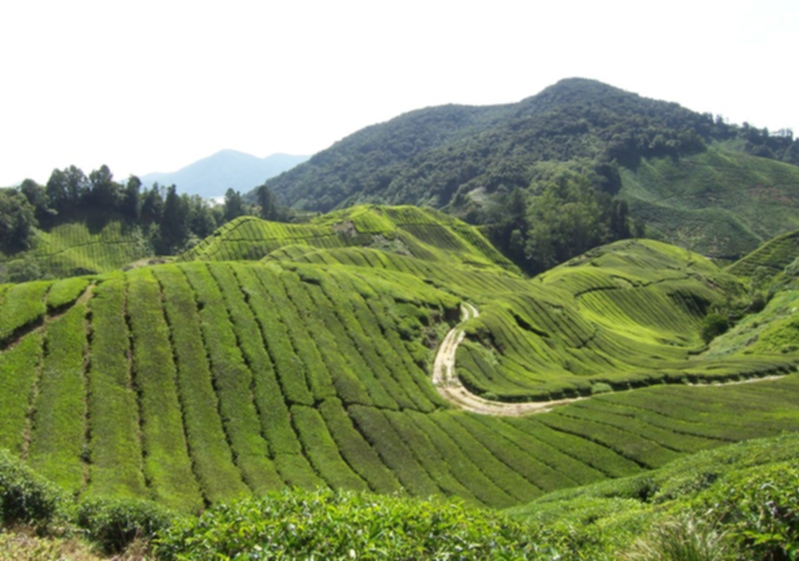
\includegraphics[width=0.382\textwidth]{pictures/tee.JPG}
  \end{center}
%\caption{A gull}
\end{wrapfigure}
In Unternehmen m\"ussen h\"aufig Entscheidungen gef\"allt werden, wie z.B. \"uber die Fertigung neuer Produkte, \"uber die Rationalisierung von Produktionsabl\"aufen, \"uber die Errichtung von Zweigwerken usw. Solche Entscheidungen k\"onnen nicht durch Probieren getroffen werden, da dies in den meisten F\"allen zu aufwendig und zu teuer --- bzw. der Zeitverlust, der durch das Probieren verursacht w\"urde --- nicht mehr vertretbar w\"are. Man versucht deshalb mathematische Verfahren als Entscheidungshilfen heranzuziehen. Ein solches Verfahren ist das lineare Optimieren. Unter \textbf{Optimierung} versteht man die Festlegung eines bestimmten Programms, mit dessen Hilfe der g\"unstigste Wert f\"ur ein vorgegebenes Ziel erreicht wird. Dabei spielen Restriktionen (Nebenbedingungen), die sich oft durch Ungleichungen ausdr\"ucken lassen, eine wichtige Rolle.

Nicht nur in der Schweiz wird sehr viel \"uber die Probleme der Energieversorgung diskutiert. Anhand dieses Problems soll das Prinzip der linearen Optimierung erl\"autert werden. In einer Region stehen verschiedene Energiequellen zur Verf\"ugung. Der Energiebedarf wird weiterhin ansteigen und man muss zus\"atzliche Kraftwerke errichten. Das Ziel der Planung heisst: Bau von Kraftwerken, die bei minimaler Belastung der Umwelt --- auch in der Zukunft ---, also minimalen Kosten, den Energiebedarf der Region decken. Verschiedene Typen (Wasser-, Kohle-, Atomkraftwerke u.a.) stehen zur Auswahl. Bei der Planung m\"ussen folgende Bedingungen beachtet werden:

\begin{itemize}
\item die Spitzenleistung der verschiedenen Kraftwerkstypen,
\item die j\"ahrliche Energiemenge, die die verschiedenen Kraftwerkstypen liefern k\"onnen,
\item die H\"ohe der Bauinvestitionen f\"ur die verschiedenen Typen,
\item die j\"ahrlichen Betriebskosten,
\item die Kosten f\"ur die Sicherheitseinrichtungen (Luftfilter, Entsorgung etc.).
\end{itemize}

\begin{bem}
Die Alternative zum K-Pfad (Kernenergie, kapitalintensive Energieproduktion und Konzentration der Erzeugungsanlagen) ist der S-Pfad. Das \glqq S\grqq\ steht f\"ur Sparen, f\"ur Sonnenenergie und f\"ur sanfte, d.h. erneuerbare Energiearten. Dass der S-Pfad machbar ist, es also auch ohne Kernenergie m\"oglich ist, den privaten Konsum weiter zu steigern, haben viele Studien nachgerechnet und belegt. Die Gesellschaft kann ohne Verlust an Lebensqualit\"at auf dem S-Pfad in eine Zukunft gehen, in der Energie umweltfreundlich, sozialvertr\"aglich und ohne Risiko produziert werden kann.
\end{bem}

An diesem obigen Beispiel erkennt man, dass eine Optimierungsaufgabe aus zwei Teilen besteht. Einmal aus dem Ziel (hier: minimale Kosten), das durch den Optimierungsprozess erreicht werden soll, zum anderen aus den Bedingungen, die das Erreichen des Ziels beeinflussen. So wird die lineare Optimierung zu einer der wichtigsten Grundlagen der Unternehmensforschung (Operations Research).

Das beste \"okonomische Verhalten muss bei bestimmten Bedingungen gefunden werden. Industrie und Handel m\"ussen daf\"ur sorgen, Produktivit\"at und Gewinn so hoch wie m\"oglich und die Kosten f\"ur die Erzeugung, Verwaltung und den Transport so niedrig wie m\"oglich zu halten. In der Praxis sind die Nebenbedingungen meist so zahlreich, dass man nur mit Hilfe von Computern die optimale L\"osung finden kann. Die heutigen Computersysteme k\"onnen Probleme mit mehreren Tausenden von Variablen und Restriktionen l\"osen. Jedes Rechenzentrum hat derartige Computerprogramme, die auf dem Simplex-Algorithmus beruhen. Dieser Algorithmus wurde erst 1950 von dem Amerikaner \textsc{Dantzig} entwickelt. Insbesondere die \"Ol-Multis haben mit dieser Methode gute Gesch\"afte gemacht, indem sie ihre Tankerflotten mit geringsten Kosten auf schnellsten Wegen zu den jeweils gewinntr\"achtigsten M\"arkten dirigierten. 1978 fand der sowjetische Mathematiker \textsc{Kachijan} ein neues Verfahren, das den im Vergleich recht umst\"andlichen Simplex-Algorithmus ersetzen wird, da es sehr viel schneller zur optimalen L\"osung gelangt und damit die Behandlung noch komplexerer Probleme (u.a. nichtlineare Optimierung) erm\"oglicht.

Wir betrachten hier verh\"altnism\"assig einfache Probleme, die sich mit graphischen Methoden l\"osen lassen: Von einer Funktion $Z$ (genannt \textbf{Ziel\-funk\-tion}) werden extremale Werte bestimmt, wobei die Nebenbedingungen (lineare Ungleichungen) zu beachten sind. Diese Bedingungen ergeben, graphisch in einem Koordinatensystem dargestellt, das sogenannte \textbf{Planungspolygon}.

\begin{bsp}
Eine Fabrik stellt die beiden Modelle \glqq analog\grqq\ und \glqq digital\grqq\ eines Taschenradios her. Jedes Radio der Analogausf\"uhrung bringt einen Gewinn von Fr. 15.-, das der Digitalausf\"uhrung Fr. 45.-.
Die Tagesproduktion der Firma unterliegt den folgenden Einschr\"ankungen: Von der Analogausf\"uhrung k\"onnen h\"ochstens 1200, von der Digitalausf\"uhrung h\"ochstens 700, von beiden zusammen h\"ochstens 1400 St\"uck hergestellt werden. In der Analogausf\"uhrung wird eine Verst\"arkerstufe, in der Digitalausf\"uhrung werden zwei Verst\"arkerstufen eingebaut. Pro Tag stehen aber h\"ochstens 1800 Verst\"arkerstufen zur Verf\"ugung.

Wie viele Analog- bzw. Digitalradios soll die Firma pro Tag herstellen, wenn ihr Gewinn m\"oglichst gross sein soll?
Werden die Anzahl der pro Tag hergestellten Analogger\"ate mit $x$ und die Anzahl der Digitalger\"ate mit $y$ bezeichnet, so k\"onnen die erw\"ahnten Nebenbedingungen (Restriktionen) als ein Ungleichungssystem formuliert werden:
\begin{align}
x&\leq1200\\
y&\leq700\\
x+y&\leq1400\\
x+2y&\leq1800
\end{align}
Ausserdem gelten noch die Bedingungen
\begin{align*}
x\geq0\\
y\geq0
\end{align*}
da ja die Anzahlen $x$ und $y$ nicht negativ sein k\"onnen.

Zun\"achst wird das \textbf{Planungspolygon}, die L\"osungsmenge des Ungleichungssystems, erstellt:
\begin{figure}[h!]
\begin{center}
\definecolor{zzttqq}{rgb}{0.6,0.2,0}
\definecolor{cqcqcq}{rgb}{0.75,0.75,0.75}
\scalebox{1}{
\begin{tikzpicture}[line cap=round,line join=round,>=triangle 45,x=0.0033cm,y=0.0033cm]
\draw [color=cqcqcq,dash pattern=on 3pt off 3pt, xstep=0.66cm,ystep=0.66cm] (-200,-196.58) grid (1920.04,1500);
\draw[->,color=black] (-200,0) -- (1920.04,0);
\foreach \x in {-200,200,400,600,800,1000,1200,1400,1600,1800}
\draw[shift={(\x,0)},color=black] (0pt,2pt) -- (0pt,-2pt) node[below] {\scriptsize $\x$};
\draw[color=black] (1878.85,13.68) node [anchor=south west] { x};
\draw[->,color=black] (0,-196.58) -- (0,1500);
\foreach \y in {,200,400,600,800,1000,1200,1400}
\draw[shift={(0,\y)},color=black] (2pt,0pt) -- (-2pt,0pt) node[left] {\scriptsize $\y$};
\draw[color=black] (12.11,1431.59) node [anchor=west] { y};
\clip(-200,-196.58) rectangle (1920.04,1500);
\fill[color=zzttqq,fill=zzttqq,fill opacity=0.1] (1.1,700) -- (400,700) -- (1000,400) -- (1200,200) -- (1200,0) -- (0,0) -- cycle;
\draw [domain=-200:1920.04] plot(\x,{(--1400-1*\x)/1});
\draw [domain=-200:1920.04] plot(\x,{(--1800-1*\x)/2});
\draw [domain=-200:1920.04] plot(\x,{(--700-0*\x)/1});
\draw (1200,-196.58) -- (1200,1500);
\end{tikzpicture}
}
\end{center}
\caption{Planungspolygon}
\end{figure}

F\"ur den Gewinn der Firma in Abh\"angigkeit von $x$ und $y$ hat man den Funktionsterm
$$G(x,y)=15x+45y.$$
$G$ heisst \textbf{Zielfunktion} und ist eine affine Funktion mit 2 Variablen. Alle Paare $\point{x}{y}$, die die obigen Bedingungen erf\"ullen, stellen zul\"assige L\"osungen des Problems dar. Gesucht wird aber dasjenige Paar $\point{x}{y}$ ($x,y$ sind nat\"urliche Zahlen), f\"ur das der Gewinn $G(x,y)$ maximal wird.

Durch Umformen des Zielfunktionsterms erh\"alt man
$$y=-\frac{1}{3}x+\frac{G}{45}$$
eine affine Funktionsschar. Die entsprechende Graphen sind parallele Geraden mit den $y$-Achsenabschnitten $\frac{G}{45}$. Gesucht ist ein Punktepaar $(x|y)$, das einerseits das Ungleichungssystem erf\"ullt, und f\"ur das andererseits der y-Achsenabschnitt $\frac{G}{45}$ und damit auch $G$ m\"oglichst gross wird.
Man erh\"alt die L\"osung $\point{x}{y}$, indem man eine Gerade der Geradenschar, etwa die durch die Punkte $(0|100)$ und $(300|0)$, $m=-\frac{1}{3}$, ausw\"ahlt, und sie solange l\"angs der y-Achse nach oben verschiebt, bis sie mit der Begrenzungslinie des Planungspolygons nur noch einen Punkt oder eine Strecke gemeinsam hat.
\begin{figure}[h!]
\begin{center}
\definecolor{zzttqq}{rgb}{0.6,0.2,0}
\definecolor{cqcqcq}{rgb}{0.75,0.75,0.75}
\scalebox{1}{
\begin{tikzpicture}[line cap=round,line join=round,>=triangle 45,x=0.0033cm,y=0.0033cm]
\draw [color=cqcqcq,dash pattern=on 2pt off 2pt, xstep=1.32cm,ystep=1.32cm] (-200,-196.58) grid (1920.04,1500);
\draw[->,color=black] (-200,0) -- (1920.04,0);
\foreach \x in {-200,200,400,600,800,1000,1200,1400,1600,1800}
\draw[shift={(\x,0)},color=black] (0pt,2pt) -- (0pt,-2pt) node[below] {\scriptsize $\x$};
\draw[color=black] (1878.85,13.68) node [anchor=south west] { x};
\draw[->,color=black] (0,-196.58) -- (0,1500);
\foreach \y in {,200,400,600,800,1000,1200,1400}
\draw[shift={(0,\y)},color=black] (2pt,0pt) -- (-2pt,0pt) node[left] {\scriptsize $\y$};
\draw[color=black] (12.11,1431.59) node [anchor=west] { y};
\draw[color=black] (0pt,-10pt) node[right] {\footnotesize $0$};
\clip(-200,-196.58) rectangle (1920.04,1500);
\fill[color=zzttqq,fill=zzttqq,fill opacity=0.1] (1.1,700) -- (400,700) -- (1000,400) -- (1200,200) -- (1200,0) -- (0,0) -- cycle;
\draw [domain=-200:1920.04] plot(\x,{(--1400-1*\x)/1});
\draw [domain=-200:1920.04] plot(\x,{(--1800-1*\x)/2});
\draw [domain=-200:1920.04] plot(\x,{(--700-0*\x)/1});
\draw (1200,-196.58) -- (1200,1500);
\draw [domain=-200:1920.04] plot(\x,{(--100-0.33*\x)/1});
\draw[smooth,samples=100,domain=-100.0:1400.0] plot(\x,{300-\x/3});
\draw[smooth,samples=100,domain=-100.0:1400.0] plot(\x,{500-\x/3});
\draw[smooth,samples=100,domain=-100.0:1400.0] plot(\x,{835-\x/3});
\draw[smooth,samples=100,domain=-100.0:1400.0] plot(\x,{700-\x/3});
\draw[color=black] (-100,80) node {$y_Z$};
\end{tikzpicture}
}
\end{center}
\caption{Zielgerade und Optimum}
\end{figure}
Wie aus der Zeichnung abzulesen ist, entpuppt sich das Paar $\point{400}{700}$ als optimale L\"osung des Problems. Die Firma erzielt einen maximalen Gewinn, wenn sie pro Tag 400 Analogradios und 700 Digitalradios herstellt. Den entsprechenden Gewinn berechnet man mit Hilfe der Zielfunktion:
$$G(400,700) = \unit[15\cdot400]{Fr.} + \unit[45\cdot700]{Fr.} = \unit[37\,500]{Fr.}$$
Die optimale L\"osung kann auch rechnerisch ermittelt werden, indem man den Schnittpunkt der beiden entsprechenden Geraden berechnet (L\"osen eines Gleichungssystems mit 2 Unbekannten).
\end{bsp}

\begin{bem}
Man h\"atte die L\"osung auch direkt erkennen k\"onnen. W\"ahlt man n\"amlich die maximale Anzahl produzierbare Digitalradios, 700, dann wird man den gr\"osstm\"oglichen Gewinn erzielen, weil die Digitalradios im Verkauf mehr einbringen als die Analogvariante. Ist dem wirklich so?
\end{bem}

\begin{ueb}
Die Konkurrenz zwingt die Firma ihren Preis f\"ur die Digitalausf\"uhrung so zu senken, dass ihr Gewinn nur noch $\unit[25]{Fr.}$ pro St\"uck betr\"agt. Wie soll die Firma reagieren?
\end{ueb}

\begin{ueb}
  Ein landwirtschaftlicher Weidebetrieb hat sich auf die Haltung von
  K\"uhen und Jungvieh spezialisiert. In den St\"allen des Betriebs
  k\"onnen h\"ochstens $70$ K\"uhe und $500$ St\"uck Jungvieh gehalten
  werden.

  \noindent F\"ur die Ern\"ahrung einer Kuh sind $0.25$ ha, f\"ur ein
  Jungvieh $0.10$ ha Weideland n\"otig. Insgesamt hat der Betrieb $50$
  ha Weideland.

  \noindent F\"ur die Pflege der K\"uhe und des Jungviehs stehen drei
  Arbeiter zur Verf\"ugung, die insgesamt $8000$ Arbeitsstunden im
  Jahr leisten. F\"ur eine Kuh sind $100$ Arbeitsstunden, f\"ur ein
  St\"uck Jungvieh $10$ Arbeitsstunden je Jahr notwendig. Der Gewinn
  bei einer Kuh betr\"agt $\unit[400]{\euro{}}$, bei einem Jungvieh $\unit[50]{\euro{}}$ im
  Jahr.

  \noindent Wie viele K\"uhe und wie viel St\"uck Jungvieh muss der
  Betrieb halten, damit der Gesamtgewinn m\"oglichst gross wird?
\end{ueb}

\subsection{Regeln zum L\"osen von Aufgaben zur linearen Optimierung}
Eine Aufgabe zur linearen Optimierung l\"ost man wie folgt:

\begin{enumerate}
  \item Annahme:
  \begin{itemize}
    \item Man stellt die gegebenen Daten tabellarisch dar
    \item und definiert die Unbekannten.
  \end{itemize}
  \item Ungleichungen:
  \begin{itemize}
    \item Man \"ubersetzt die im Aufgabentext umschriebenen
    Bedingungen in die Formelsprache der Mathematik.
  \end{itemize}
  \item Planungspolygon:
  \begin{itemize}
    \item Man stellt die L\"osungen des Ungleichungssystems graphisch
    dar.
  \end{itemize}
  Dabei verwendet man folgende Tatsachen:
  \begin{itemize}
    \item Punkte, deren Koordinaten $\point{x}{y}$ die Ungleichung $y>mx+b$
    bzw. $y<mx+b$ erf\"ullen, bilden eine Halbebene, die oberhalb bzw.
    unterhalb des Graphen der Funktion $y=mx+b$ liegt.
    \item Der mengentheoretische Durchschnitt aller Halbebenen, die
    sich aus den Ungleichungen ergeben, bilden das sogenannte
    Planungspolygon.
  \end{itemize}
  
  \pagebreak
  
  \item Zielfunktion:
  \begin{itemize}
    \item Man dr\"uckt die Gr\"osse $z$, die optimal werden soll, mit
    den Unbekannten aus.
    \item Man l\"ost die Gleichung nach $y$ auf
    \item und zeichnet den zugeh\"origen Graphen f\"ur ein frei
    w\"ahlbares $z$ im gleichen Koordinatensystem wie das
    Planungspolygon ein.
  \end{itemize}
  \item Optimum:
  \begin{itemize}
    \item Man untersucht, welche Parallele zur Zielgerade das
    Planungspolygon in mindestens einem Punkt $P$ schneidet und ein
    optimales $z$ liefert.
    \item $P$ ist der optimale Punkt; man berechnet seine
    Koordinaten.
    \item Falls die Koordinaten von $P$ nicht ganze Zahlen sind, die
    gesuchten Unbekannten jedoch ganzzahlig sein sollten, muss man
    die Umgebung von $P$ in einer zus\"atzliche Skizze vergr\"ossert
    darstellen, damit man gegebenenfalls richtig runden kann.
  \end{itemize}
  \item Antwort:
  \begin{itemize}
    \item Man liest die Aufgabenstellung erneut.
    \item Man beantwortet die gestellten Fragen mit einem Text.
  \end{itemize}

\end{enumerate}

\begin{center}
Stichwort $\rightarrow$ \texttt{AUPZOA}
\end{center}

\subsection{Weitere \"Ubungen}
\begin{ueb}
  Zur Erhaltung seiner Gesundheit ben\"otigt der Mensch w\"ochentlich
  mindestens $\unit[70]{mg}$ Vitamin H und $\unit[150]{mg}$ Vitamin B. In einer
  Apotheke gibt es Tabletten, von denen die eine Sorte $\unit[10]{mg}$ H und
  $\unit[30]{mg}$ B je Gramm enth\"alt, die andere $\unit[20]{mg}$ H und $\unit[10]{mg}$ B.
  Die erste Sorte kostet $50$ Rappen pro Gramm, die zweite $40$
  Rappen pro Gramm. Wie viel Gramm von jeder Sorte w\"are w\"ochentlich
  n\"otig, um den Bedarf auf diese Weise mit m\"oglichst geringen Kosten
  zu decken?
\end{ueb}

\begin{ueb}
Einer Forschungsexpedition stehen in ihren Beh\"altern $\unit[21\,600]{cm^3}$ f\"ur Batterien f\"ur das Funkger\"at zur Verf\"ugung. Der Expeditionsleitung werden zwei Sorten von Batterien gleicher Leistung mit den Gr\"ossen $\unit[200]{cm^3}$ und $\unit[300]{cm^3}$ angeboten. Die Batterien kosten $\unit[10]{Fr.}$ bzw. $\unit[5]{Fr.}$ pro St\"uck. Mehr als $\unit[500]{Fr.}$ darf man f\"ur den Batteriekauf aber nicht ausgeben. Die Batterie der ersten Sorte h\"alt 18 Stunden, die der zweiten Sorte 16 Stunden. Wie viele Batterien jeder Sorte sollen eingekauft werden, damit die Funkanlage m\"oglichst lange benutzt werden kann?
\end{ueb}

\begin{ueb}
Die Bepflanzung einer Hektare Ackerland mit Kartoffeln erfordert einen Arbeitsaufwand von einem Tag und Kosten von $\unit[10]{Fr.}$, diejenige mit Getreide einen Arbeitsaufwand von 4 Tagen und $\unit[20]{Fr.}$ Kosten. Der Ertrag einer Hektare Kartoffelacker betr\"agt $\unit[40]{Fr.}$ und derjenige einer Hektare Getreideacker $\unit[120]{Fr.}$. Ein Bauer besitzt einen Acker von 100 Hektaren, hat $\unit[1100]{Fr.}$ zur Verf\"ugung und rechnet mit 160 Arbeitstagen. Wie viele Hektaren muss er mit Kartoffeln, wie viele mit Getreide bepflanzen und wie viele muss er brach liegen lassen, damit der Gesamtertrag m\"oglichst gross wird? Wie hoch wird sein Gesamtertrag?
\end{ueb}

\begin{ueb}
Ein Mensch braucht pro Tag $\unit[70]{g}$ Eiweiss, $\unit[60]{g}$ Fett, $\unit[400]{g}$ Kohlenhydrate. Ein Brot enth\"alt pro $\unit[100]{g}$ $\unit[10]{g}$ Eiweiss, $\unit[4]{g}$ Fett und $\unit[40]{g}$ Kohlenhydrate. Eine Schokolade enth\"alt pro $\unit[100]{g}$ $\unit[8]{g}$ Eiweiss, $\unit[30]{g}$ Fett und $\unit[60]{g}$ Kohlenhydrate. Stelle ein Nahrungsmittelpaket mit minimalem Gewicht zusammen, das jeweils von den genannten N\"ahrstoffen wenigstens die t\"agliche Mindestmenge enth\"alt. Wie gross wird dieses Minimalgewicht?
\end{ueb}

\begin{ueb}
Eine Fleischfabrik verfrachtet t\"aglich $\unit[17\,800]{kg}$ Frischfleisch und $\unit[11\,000]{kg}$ tiefgek\"uhltes Fleisch an verschiedene Metzgereien. F\"ur den Versand stehen 2 Typen von Lieferwagen zur Verf\"ugung:

\begin{description}
\item[Typ I] $\unit[600]{kg}$ Frischfleisch, $\unit[300]{kg}$ tiefgek\"uhltes Fleisch,
\item[Typ II] $\unit[500]{kg}$ Frischfleisch, $\unit[400]{kg}$ tiefgek\"uhltes Fleisch
\end{description}

Die Transportkosten pro km betragen beim Typ I 4 Franken, beim Typ II 4.80 Franken. Wie viele Wagen jeden Typs sollten eingesetzt werden, um die Transportkosten m\"oglichst niedrig zu halten? Wie hoch sind diese Transportkosten?
\end{ueb}

\begin{ueb}
An einer Stassenkreuzung gibt die Ampel A zwei Fahrspuren, die Ampel B drei Fahrspuren frei. Aufgrund der Ergebnisse von Verkehrsz\"ahlungen soll die Gr\"unphase von B l\"anger als die von A, aber weniger als doppelt so lang als die von A sein. Es wird angenommen, dass durchschnittlich ein Fahrzeug pro Sekunde auf jeder Fahrspur an jeder Ampel vorbeif\"ahrt. Wegen der Fussg\"anger sollen beide Gr\"unphasen zusammen nicht l\"anger als 60 Sekunden
betragen. Wie m\"ussen die beiden Ampeln geschaltet werden, damit in den Gr\"unphasen m\"oglichst viele Fahrzeuge die Kreuzung passieren k\"onnen? Wie viele Fahrzeuge k\"onnen in den Gr\"unphasen maximal die Kreuzung passieren?
\end{ueb}

\clearpage
\listoffigures
%\listoftables
%\newpage
%\nocite{*}
%\bibliographystyle{plain}
%\bibliography{preamble/literaturgoogle}
\end{document}